
\newpage
\section{Flabby Flame - Unity3D\\{\small \emph{Dilan Perale}}}
\label{sec:unity}

La sezione su Unity è stata strutturata seguendo quasi passo per passo ciò quello che un developer fa inizialmente per affrontare questo ambiente. Si inizia, quindi, dall'installazione di Unity, per poi andare a vedere le varie guide, i tutorial e cosa offre la community. Ci si scontra poi con l'interfaccia grafica, le principali componenti di Unity e il suo editor per gli script, che serviranno a governare il gioco. Si va, infine, a costruire l'applicazione per le varie piattaforme. Dopo aver enunciato questi aspetti, lo scrivente dettaglia nella parte centrale della relazione le peculiarità del gioco realizzato con Unity, i suoi bug e la sua usabilità. Infine nella parte conclusiva, si descrivono le varie impressioni, positività e criticità sul codice e su Unity stesso.

\subsection{Installazione}

L’installazione di Unity avviene tramite eseguibile ed è durante il procedimento di installazione che si scelgono i vari componenti da installare. Risulta essere un framework alquanto pesante soprattutto se si vanno a sommare i diversi contenuti opzionali. Considerato poi che la velocità della linea internet incide sulla durata dell’installazione, ne consegue che il tempo necessario per la stessa può essere più o meno lungo.
Per quanto concerne il suddetto progetto, si è verificato un unico problema al primo avvio di Unity dopo l’installazione su computer desktop, ovvero si è aperta una schermata bianca (si veda figura 1). Lo scrivente ha risolto la questione in tempi brevi grazie ad una guida realizzata da un utente che aveva fronteggiato il medesimo problema. La seconda installazione su dispositivo laptop, invece, è andata subito a buon fine.

\begin{figure}[h]
\centering
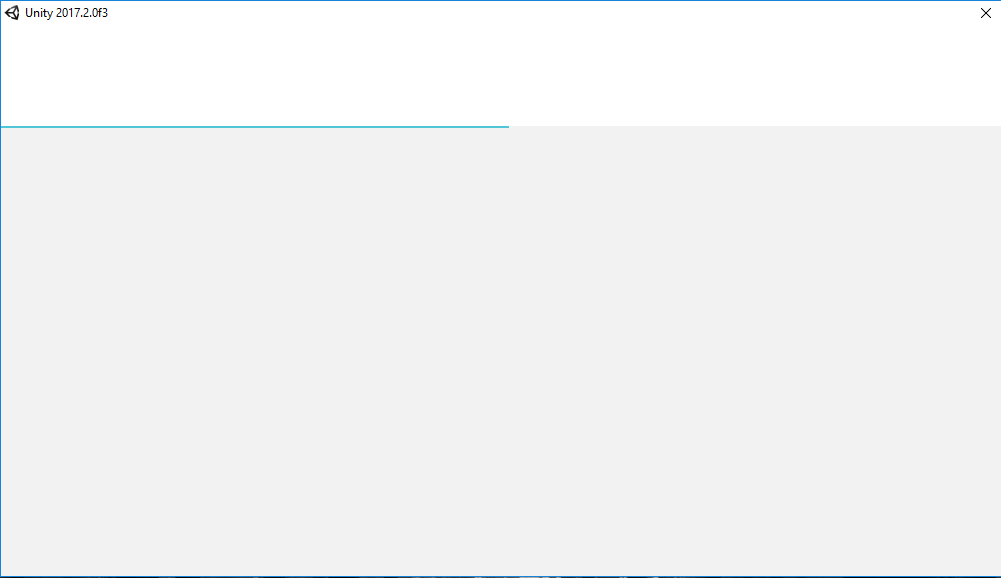
\includegraphics [width=\textwidth]{img/unity_problem.png}
\caption{\label{fig:problem} Problema Unity.}
\end{figure}

\subsection{Documentazione, community e tutorial}

Lo scrivente ha contattato l’assistenza Unity per approfondire il problema che si era verificato durante l’installazione su Desktop: essa ha risposto tempestivamente al quesito, fornendo le informazioni necessarie per proseguire il lavoro. Questo riscontro ha sottolineato un punto di forza del framework.
Si sottolinea che anche la documentazione per le classi specifiche di Unity e i GameObject è molto dettagliata e che, in caso di difficoltà di comprensione, viene subito in aiuto la community di Unity. Quest’ultima è molto vasta ed esperta e proprio per queste sue caratteristiche fornisce le risorse che permettono all’utente di risolvere i problemi riscontrati molto velocemente.
Infine, sono veramente ottimi i vari tutorial che fornisce il sito di Unity, poichè spiegano dettagliatamente come funzionano le varie parti del framework e affrontano gli aspetti principali dei giochi più basici, permettendo all’utente di creare fin da subito un lavoro concreto. Inoltre, si mette in evidenza che ci sono innumerevoli tutorial accurati fatti dagli stessi utenti di Unity che forniscono un grande aiuto a colui che vuole utilizzare il framework.

\subsection{Interfaccia grafica}

L’interfaccia grafica di Unity è molto intuitiva, completa e altamente personalizzabile. Ogni parte di Unity ha il suo pannello di visualizzazione che permette di spostare le varie parti in più schermi e può essere posizionato a piacimento sia all’interno dell’interfaccia principale sia all’esterno.
Lo scrivente ha costruito, quindi, la sua l’interfaccia personalizzandola in base alle esigenze del progetto. In questa fase ne ha selezionato sei parti: visualizzazione delle directory del progetto, scene e sue componenti, visualizzazione delle suddette, emulatore, inspector e animator. L’emulatore può essere portato a full screen all’avvio ed è utilizzato per provare le scene, l’inspector viene impiegato per ispezionare le caratteristiche dell’elemento selezionato, mentre l’animator è adoperato per creare animazioni. Di seguito, in figura 2, si può osservare l’immagine dell’interfaccia dello scrivente in seguito alla personalizzazione.

	\begin{figure}[h]
	\centering
	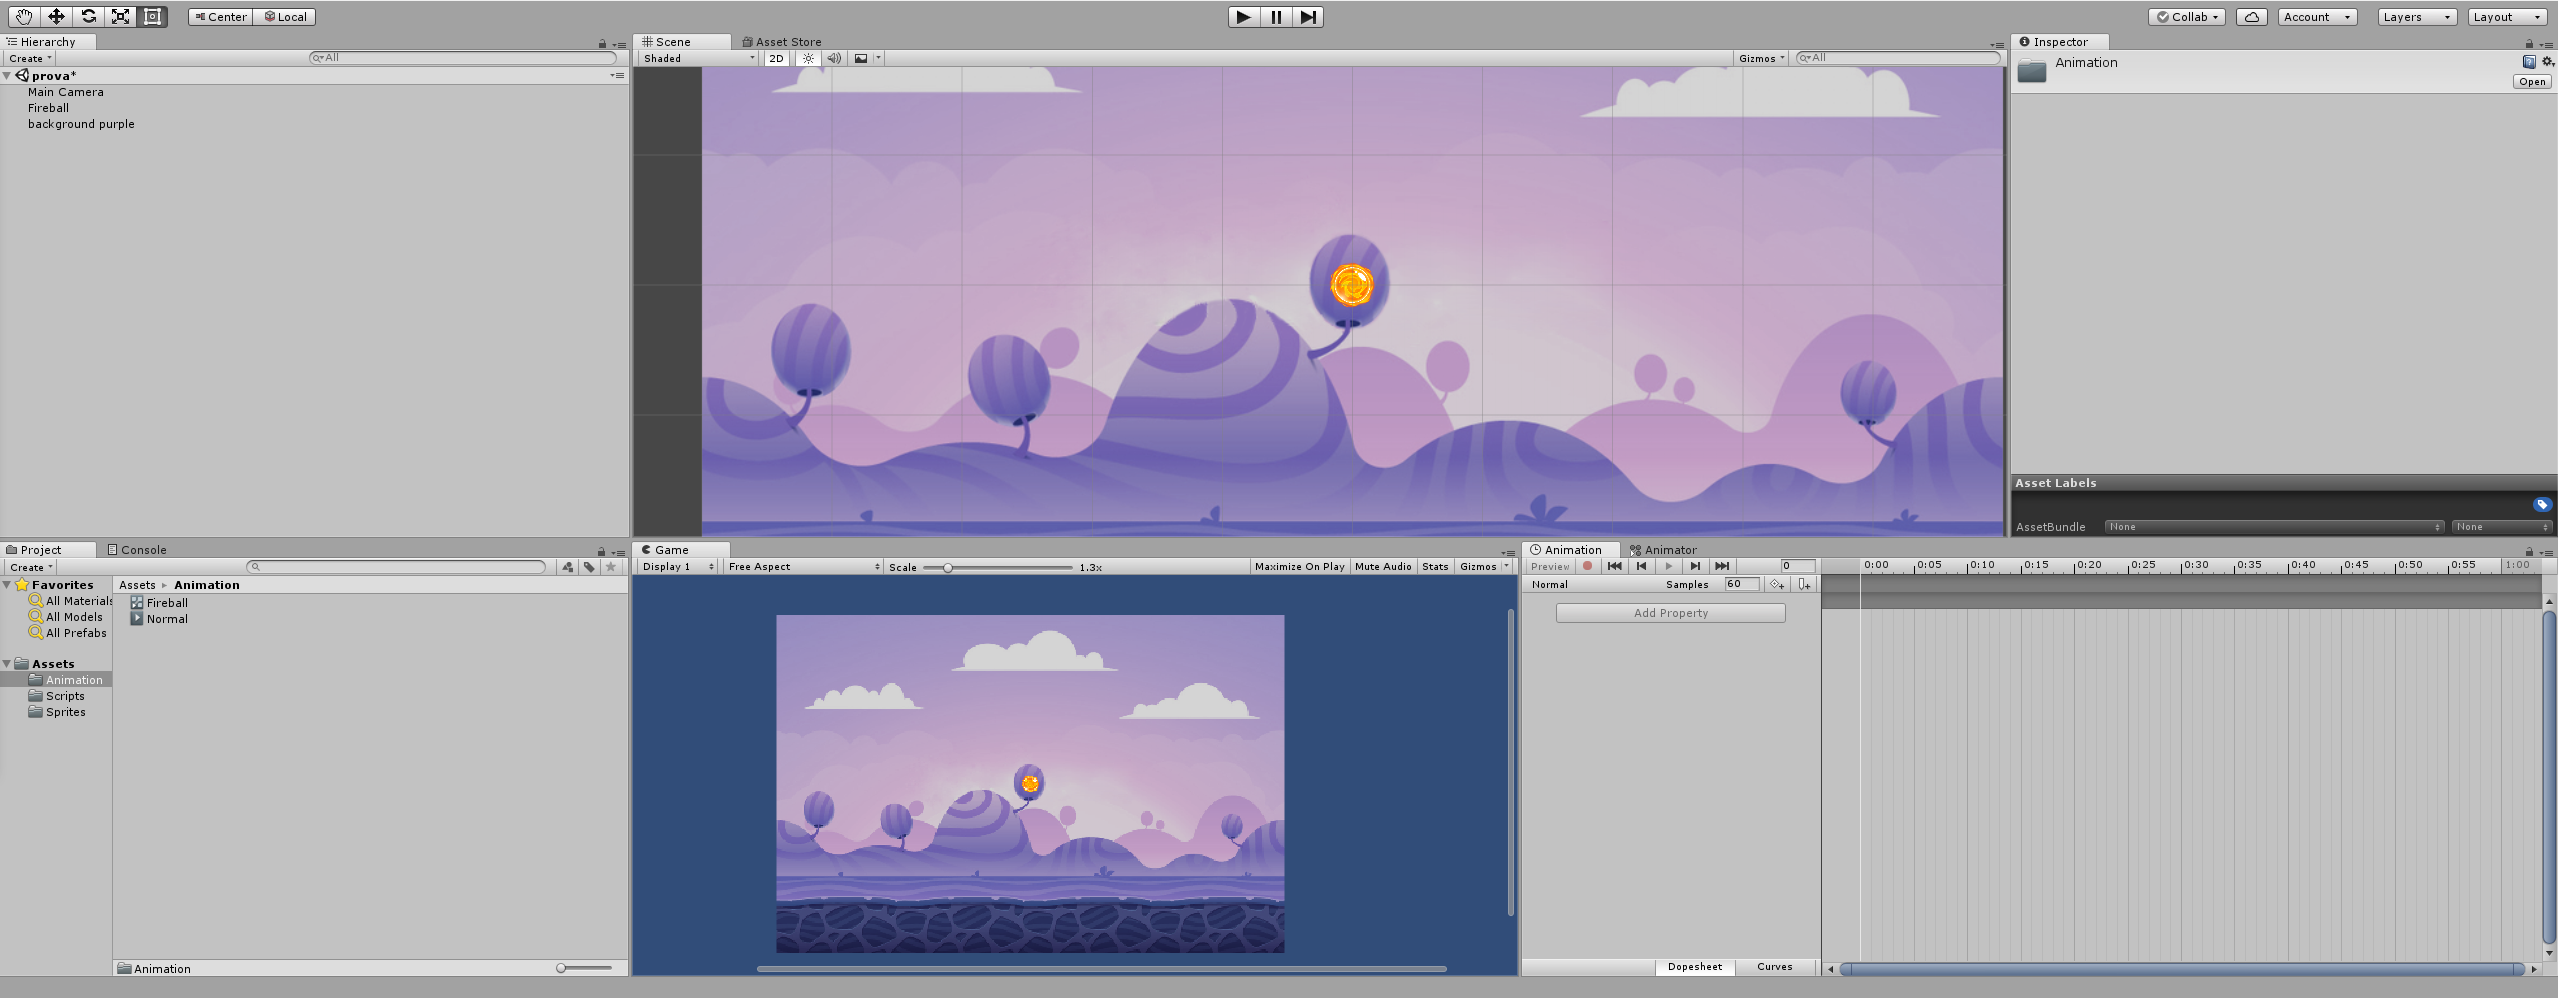
\includegraphics [width=\textwidth]{img/Unity_organizzazione.png}
	\caption{\label{fig:interface} Interfaccia Unity personalizzata.}
	\end{figure}

\subsection{Principali componenti e MonoDevelop}

La suddivisione di un gioco in Unity è definito dalle scene che contribuiscono a formare un determinato spazio di gioco. Le scene sono un insieme di GameObject che possono essere visibili all’utente che fruisce dell’applicazione, come la telecamera, il background e il terreno, ma che possono anche non essere riconoscibili dallo stesso, sebbene siano di fondamentale importanza per la riuscita del gioco: ne sono un esempio i box per le collisioni.
Tra i GameObject ci sono gli oggetti per la UI (User Interface), ovvero l’audio, i video, le luci e gli effetti. Per governare le varie interazioni tra oggetti, movimenti e quant’altro si ha poi bisogno di un altro elemento, che si va ad affiancare all’interfaccia grafica di Unity che, seppur ottima e completa, non permette all’utente di effettuare tutte le operazioni che desidera. Questo elemento, o meglio, questi elementi, sono gli script che possono essere scritti in C\#  o JavaScript. Per scrivere gli script si può adoperare un IDE qualsiasi compatibile con questi linguaggi, come Visual Studio, ma Unity mette anche a disposizione un suo editor, MonoDevelop. Si tratta di un editor completo, seppur con ancora qualche bug, facilmente personalizzabile e che possiede un debugger.
Comunque, a prescindere dall’editor utilizzato, si mette in evidenza che gli script hanno un diagramma di flusso del ciclo di vita molto complicato, ma nello stesso tempo organizzato: ne deriva che, inizialmente, affrontarlo non è facile e si incappa in molti errori per le tempistiche di esecuzione degli script stessi.

\subsection{Build}

È possibile fare una build della propria applicazione su molte piattaforme diverse, quali PC, Android, IOS, PS, XBOX e Facebook. Si specifica che, per quanto concerne la predisposizione di questo progetto, lo scrivente ha provato le piattaforme PC e Android, mentre la build per IOS è stata solo studiata.
Durante l’installazione di Unity, si scelgono e scaricano le componenti aggiuntive, ma a differenza di Android e IOS, per la piattaforma PC, queste sono già preinstallate.
A questo punto, una volta creata l’applicazione, o almeno un qualcosa di eseguibile, si può fare la build: quella per il PC si crea senza alcun problema, mentre per quanto riguarda le altre due piattaforme si deve prima preparare l’ambiente. Per fare questo, sia per Android che IOS, il developer può usufruire di guide.
\paragraph{Android}
Se si considera la prima piattaforma si devono scaricare gli SDK tools e poi installare i pacchetti per la versione Android che si desidera. Lo scrivente non ha riscontrato significativi problemi, se non un malfunzionamento degli SDK tools: per far fronte a questa lieve complicazione si è scaricato l’intero Android Studio. Successivamente si è cambiata la versione dei tools e si è messa quella precedente. Infine, venivano richieste da Unity le JDK, ma anch’esse nell’ultima versione davano dei problemi, perciò, anche in questo caso, si è scaricata una versione antecedente. Per l’intero procedimento si è persa più di un’ora di tempo, ma, messe le ultime impostazioni richieste, si è alla fine riusciti a far andare l’applicazione su uno smartphone.
\paragraph{iOS}
Per iOS il procedimento è completamente diverso a quello appena descritto. Esistono due strade che l’utente può percorrere.
Considerata la prima, il programmatore ha bisogno di un MAC, di un account Apple da developer e di Xcode installato. La build di Unity creerà un progetto Xcode dal quale poi si potrà realizzare una build per il dispositivo IOS. Questo metodo è complicato per chi non dispone di un MAC, poiché le alternative sono degli emulatori della piattaforma o cose simili.
L’altro procedimento per fare la build per IOS è usare Unity Cloud Build che permette ad un intero team di poter condividere online la build e poterla usare sui vari dispositivi. Questi ultimi possono essere anche diversi da IOS, essendoci una build per ogni piattaforma interessata. Unity Cloud Build va, quindi, incontro e facilita le interazioni tra i membri di un team. Si osserva che sebbene la versione gratuita è molto limitante, il prezzo per la versione pro è veramente ridotto per le potenzialità che offre. Tuttavia, questo metodo non risolve totalmente il problema con IOS, poiché un account Apple da developer è sempre necessario e perché per poter non utilizzare un MAC, sempre se sia possibile (si specifica che lo scrivente non ha provato questo passaggio), si devono seguire rigide guide.


\subsection{Applicazione Unity}
\subsubsection{Menu principale}
L’applicazione si apre su un menu principale costituito da 5 pulsanti:
\begin{enumerate}
\item Play: fa partire il gioco. Se il gioco viene aperto per la prima volta, l’utente visualizzerà un mini-tutorial per capire le funzioni dell’applicazione;
\item Options: tasto che offre le impostazioni principali del gioco, cioè il volume e la personalizzazione della pallina;
\item Coppa, Best score: permette di osservare il punteggio migliore;
\item Punto interrogativo, Help: fornisce la spiegazione del gioco;
\item Porta, Exit: consente l’uscita dall’applicazione.
\end{enumerate}
Ora una breve descrizione sulla sua usabilità. Il gioco deve sicuramente essere giocabile ma anche il suo menu deve essere usabile. In questo caso ci vogliono degli accorgimenti, che in parte sono stati implementati e in parte solo descritti. 
Il menu ha tasti abbastanza grandi per poter essere cliccati con facilità. Il tasto “exit” è posizionato nel punto più difficoltoso da tappare per l’utente così che lo stesso non rischi di premerlo per sbaglio. Si deve considerare però che l’implementazione del menu poteva, e magari doveva, essere fatta diversamente per mobile. Il tasto di uscita non è necessario, poichè è possibile uscire direttamente con i tasti già forniti dal sistema operativo: in ambiente Android è importante visualizzarne i tasti principali. Anche lo Slider del volume si può togliere, ma quest’ultimo è stato implementato per poter affrontare l’argomento Slider. 
Quindi, il menu poteva essere costruito senza pulsante “exit”, ma, al suo posto, con un tasto che attivava/disattiva l’audio. A questo punto il tasto “options” diventa inutile avendo una sola voce: in questo caso si potrebbe inserire nel menu principale il pulsante “customize” al suo posto.
 
\subsubsection{Gameplay}
Quando l’utente preme il tasto “play”, il gioco inizia. L’interfaccia dell’applicazione consiste in una pallina a cui è applicata la forza di gravità e una forza contraria in caso di click o tap dello schermo. Il background scorre insieme a delle stalagmiti che fuoriescono dall’alto e dal basso dello schermo: scopo del gioco è di evitare di colpire le stalagmiti e di non toccare né il pavimento né il cielo. Il giocatore perde la partita se sfiora una di queste parti.
Si sottolinea la presenza di un pulsante “options” a forma di ingranaggio nella schermata principale, che, in caso in cui sia premuto, fa comparire il menù principale e mette il gioco in pausa. Quando il player lo schiaccia per la prima volta, lo stesso vedrà un tutorial che spiegherà la possibilità di scuotere il telefono per mettere in pausa il gioco più facilmente e in modo alternativo.

\subsubsection{Bug riscontrati}
\begin{enumerate}
\item Tenendo premuto, anche per un breve lasso di tempo, una qualsiasi zona dello spazio di gioco non appena si muore si ha un bug: se il colore della pallina non è quello predefinito si avrà una fusione tra due colori e l’animazione non andrà più nella successiva partita.Presente solo su piattaforma android.
\item Se il colore non è quello predefinito ad ogni inizio partita avverrà il cambio solo dopo un update. Bug presente su Android, PC, emulatore Unity
\end{enumerate}

Si specifica che il colore è un problema di implementazione dovuto al fatto di non aver utilizzato un metodo appropriato per questo tipo di operazione. Il procedimento corretto prevedeva alcune componenti grafiche aggiuntive che era necessario imparare per poterle adoperare, ma che lo scrivente non riteneva fossero utili ai fini di questo progetto. Inoltre nell’ambiente PC è presente il tutorial dello shake, che però ovviamente non ha senso in questa piattaforma. Infine alcuni elementi grafici non hanno un dettaglio abbastanza alto per grandi schermi e quindi sgranano un po'.



\subsection{Valutazione finale}

\subsubsection{Diversità tra le varie piattaforme}
Se si usano le classi specifiche di Unity per riconoscere il click, il tap nell’ambiente touch può essere riconosciuto e avere le stesse funzionalità del click sinistro del mouse nell’ambiente desktop. Si tratta di un aspetto che va sicuramente a favore del framework, poiché facilita la gestione tra due diversi tipi di input. La gestione, però, non è completa dal momento che si deve tenere conto degli altri tasti del mouse e delle varie gesture che si possono fare su uno smartphone.

\subsubsection{Criticità del codice}
Utilizzando il codice è possibile usufruire di tutte le funzioni che si possono adoperare anche tramite interfaccia grafica, ma con il codice ci sono funzionalità aggiuntive che vanno gestite solo tramite esso. In questo caso di studio, le implementazioni da fare nella maggior parte dei casi sono state semplici, ma non sempre la gestione delle librerie di Unity e del suo game flow è risultata facile.Cambiare scene, mettere in pausa, muovere oggetti, gestire collisioni e interazioni da parte dell’utente sono tutte cose fattibili se prese singolarmente. Diverso, e, quindi, più complicato, è fare in modo che dopo una determinata interazione si verifichi esattamente una precisa azione, poiché le subroutine, intese come funzioni che avvengono dopo un click o dopo uno specifico evento, vengono eseguite dopo l’update che avviene ad ogni frame. 
Un esempio in questo caso di studio è la volontà di mettere in pausa dopo aver cliccato il pulsante apposito. Una volta premuto veniva eseguito l’update che rilevava un click nello spazio di gioco e di conseguenza applicava una forza alla pallina, che non era voluta. Questo problema è stato risolto dopo varie ore, e in un modo, secondo la visione dello scrivente, alquanto insoddisfacente. Semplicemente se il click avviene nello spazio del pulsante alla pallina non verrà applicata alcuna forza, questo perchè non è stato possibile capire, nell’esecuzione dell’update, che era stato schiacciato il pulsante, ma solo successivamente. Altra criticità del codice è l’uso di variabili pubbliche e classi pubbliche in C\# che a volte sono utili per non riscrivere il codice, ma che non sempre funzionano come ci si aspetta. Questo è dovuto molto probabilmente ad una scarsa conoscenza da parte dello scrivente del linguaggio e dell’ambiente Unity, ma che fa alzare la curva di apprendimento iniziale.


\subsubsection{Criticità generali su Unity}
Unity presenta alcune criticità:

\begin{enumerate}
\item Essendo un ambiente pesante, ad ogni modifica di uno script l’ambiente Unity ha qualche secondo di blocco;
\item L’emulatore interno non è sempre reattivo e, quindi, l’avvio dell’applicazione può non essere velocissima;
\item L’interfaccia grafica pur essendo molto completa, non sempre è utile nelle operazioni: ad esempio nella posizione dei box2D. Possono essere posizionati dove si vuole, ma il ridimensionamento degli stessi va ad aumentare o diminuire le dimensioni del box2D ambo i lati. Quindi se si posiziona il box alla coordinata x=0 da un lato e x=1 dall’altro, e lo si va ad allargare dalla parte destra quindi sul lato che sta a coordinate x=1 si noterà che l’allargamento non si verifica solo a destra ma anche a sinistra spostando il lato di sinistra dalla coordinata x=0. Il modo per risolvere questa cosa velocemente è sapere il numero di pixel formato dall’immagine con cui si sta lavorando.
\item Tra gli script e l’ambiente Unity non sempre c’è coerenza e cooperazione: per esempio i numeri negativi nello script venivano interpretati come positivi in Unity;
\item Bisogna porre attenzione alle trasparenze nelle immagini, soprattutto nei pulsanti, che potrebbero non essere cliccabili nelle zone di trasparenza interne quando invece si vuole che lo siano;
\item Una parte molto difficile è la gestione completa delle UI con diversi tipi di schermo: se da un lato Unity permette di farlo e mette a disposizione moltissime feature per questa operazione, dall’altro la gestione non è per niente immediata ed è di complicata comprensione.
\end{enumerate}
